\documentclass[a4paper,ngerman]{scrartcl}
\renewcommand{\rmdefault}{cmr}
\renewcommand{\sfdefault}{cmss}
\renewcommand{\ttdefault}{cmtt}
\usepackage[T1]{fontenc}
\usepackage[utf8]{inputenc}
\usepackage{array}
\usepackage{refstyle}
\usepackage{float}
\usepackage{enumitem}
\usepackage{amsmath}
\usepackage{euler}
\makeatletter
\usepackage{multirow}
\usepackage{isotope}
\usepackage{tikz-uml}
\usepackage[section]{placeins}
\flushbottom
\usepackage{geometry}
\geometry{a4paper}
\usepackage[headsepline]{scrpage2}
\usepackage{color}
\usetikzlibrary{circuits.ee.IEC}
%\usepackage{beramono}

\makeatother
%\usepackage{babel}
\usepackage{listings}
\lstset{language=verilog,
basicstyle={\footnotesize\fontfamily{fvm}\selectfont},
commentstyle={\textit},
keywordstyle={\bfseries},
tabsize=4,
frame=leftline,
numbers=left,
numberstyle={\tiny}}

\title{MIX Manual}

\author{Michael Schröder}
\begin{document}
\maketitle
\section{MIX-fpga}

Have you ever heard of Don Knuths (hypothetical) first polyunsaturated computer MIX, the 1009? In this project we will build a binary version of the MIX-Computer as described in "The Art of Computer Programming, Vol. 1" by Donald E. Knuth running on an fpga-board.

The presented implementation is based on the fpga development board iCE40HX8K-EVB from the company Olimex Ltd., which has the nice property of being completely open source. The whole project uses only FOSS free and open source hard- and software, so everybody can build their own MIX following the instructions in `build`
\begin{figure}[H]
	\centering
	\includegraphics[width=0.7\linewidth]{../MIX_toast.jpg}
	\caption{The real MIX made of atoms insted of bits.}
	\label{fig:mixtoast}
\end{figure}

\subsection{inside}

The MIX computer is composed of two little boards.
\begin{enumerate}
	\item iCE40HX8K-EVB, the fpga development board from olimex.com	
	\item  USB-serial adapter. Used to power the board with 5V and to in-/output data over serial interface.
\end{enumerate}

\begin{figure}[H]
	\centering
	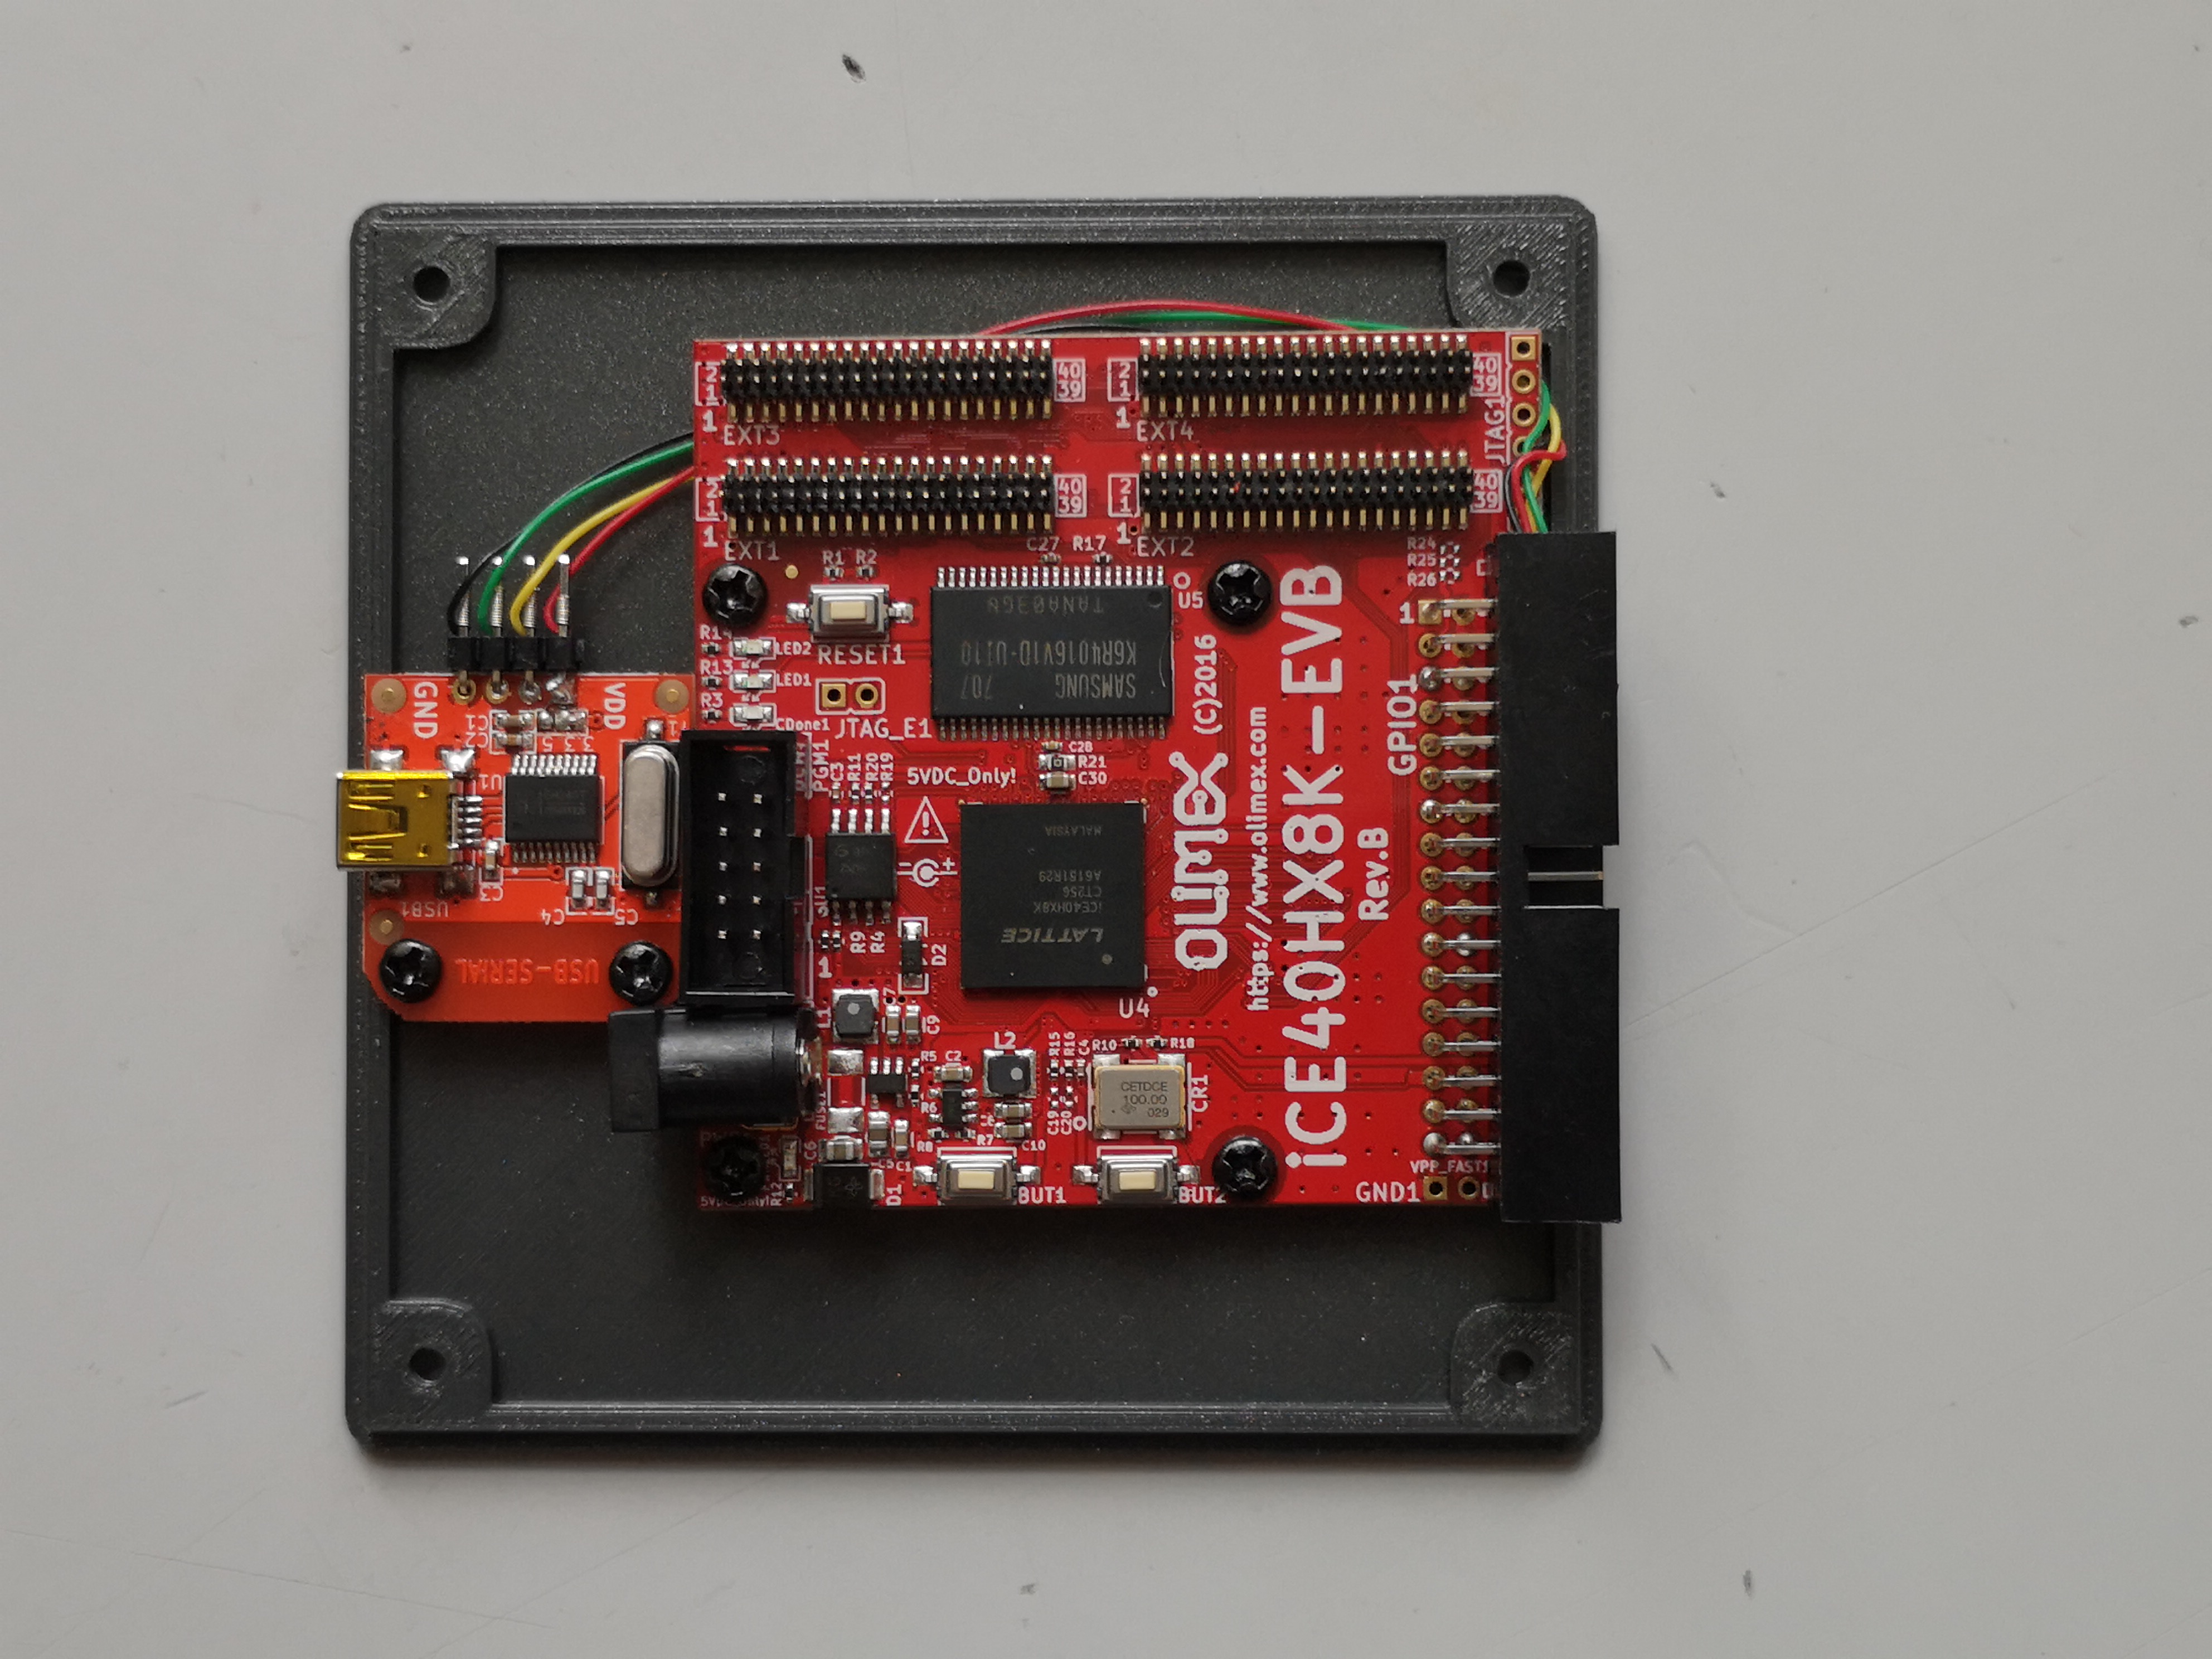
\includegraphics[width=0.7\linewidth]{../MIX_inside.jpg}
	\caption{Watch inside and see the two boards interconnected with wire wrap technique}
	\label{fig:mixinside}
\end{figure}


\subsection{Specifications}

\subsubsection{clock}
MIX runs on iCE40HX8K-EVB clocked at 25MHz. The basic unit of time 1u corresponds to 40ns, so according to Knuth it's a relatively high priced machine.

\subsubsection{I/O units}
In our MIX implementation all character based I/O units (U16-U20) are connected to the USB-connector and can be accessed as UART streams. You can connect MIX with any PC running a terminal emulator (e.g. screen for linux). The terminal should be set to 115200 baud (8N1). A conversion between ASCII and Knuths character codes is done in hardware according to Knuths specification (see TAOCP p. 128).
\begin{figure}
	\centering
	\includegraphics[width=0.7\linewidth]{../MIX_usb.jpg}
	\caption{All I/O is done through a USB to serial adapter @115200 baud}
	\label{fig:mixusb}
\end{figure}




\subsubsection{commands}
All commands exept the floating point arithmetic are implemented with execution times corresponding to Knuth's specifications. Special care is given to the correct timings. Even the "sofisticated" commands SRC and SLC, which need a modulo 10 computation are executed in the defined timing of two cycles. The system can (easily) be extended in various ways:
\begin{enumerate}
	\item add more commands:
	\begin{itemize}
		\item easy: logic operators (AND,OR,XOR,NOT)
		\item not so easy: Floating point arithmetic
		
	\end{itemize}
	\item  add more hardware:
	\begin{itemize}
		\item easy: add leds to run the traffic light example
		\item not so easy: add more I/O units
	\end{itemize}
	
	\begin{figure}[H]
		\centering
		\includegraphics[width=0.7\linewidth]{../MIX_gpio.jpg}
		\caption{MIX can be expanded through a GPIO connector placed at the read side.}
		\label{fig:mixgpio}
	\end{figure}
\end{enumerate}
\subsubsection{The GO button}
MIX comes with the \textit{GO button} attached to USB-UART. So after pressing the GO button MIX-programms can be uploaded by sending the \textit{punched cards} to USB-UART.

\subsubsection{The toast case}
MIX comes in a nice case with formfactor of a slice of toast, so your complete MIX computer system will easily fit into your lunch box. The case can be printed with a 3D printer. Design files can be found in the directory `build/toast`.
\begin{figure}[H]
	\centering
	\includegraphics[width=0.7\linewidth]{../MIX_top.jpg}
	\caption{MIX comes in the practical formfactor of a toast}
	\label{fig:mixtop}
\end{figure}


\subsubsection{Service}
In case you find encounter an issue with MIX:
\begin{itemize}
	\item don't panic
	\item send me an email to mi.schroeder@netcologne.de
\end{itemize}

\section{Running programs on MIX}
\subsection{mixasm}
To run mixal programs with MIX you first have to translate the mixal programs to machine language. This is done with the GNU tansloator `mixasm` distributed with the mix software package  `mdk`. Append the option `-l` to create a listing file `.mls`.
\subsection{tools}
To upload the code onto MIX we have to write the listing in a computer readable format. For this you can use the python scripts provided in `tools`:
\begin{itemize}
	\item \lstinline|mls2card.py|: translate the machine code (.mls) to punchcard format.
	\item  \lstinline|mls2char.py|: translate to character codes, which can directly be read by MIX. (This is only necessary for the bootloader written on the first two punch cards).
	\item  \lstinline|mls2bin.py|: translate the .mls file to binary. This is only necessary for the go-button, which must be uploaded into fpga ROM.
	 
\end{itemize}

\subsection{upload and run}
Finally you can connect to MIX with USB using a terminal emulator (screen)
\begin{lstlisting}
screen /dev/ttyUSB0 115200
\end{lstlisting}

Within  a screen session you can upload the mixal programs written on punch cards:
\begin{lstlisting}[language=bash,numbers=none]
ctr-a : readreg p p.card
ctrl-a : paste p
\end{lstlisting}


\subsection{The following programms have been tested on MIX:}

Details can be found in the README.md files found in the subfolders:
\begin{itemize}
	\item `p`: compute the first 500 primes
	\item `e`: compute easter dates
	\item  `t`: control traffic signals
	\item  `go`: the go button
	\item `boot`: the bootloader
	 
\end{itemize}

\section{program p}
We will run programm p of chapter 1.3.2 TAOCP (p. 148) on MIX. Programm p computes the first 500 primes and outputs them in a table on the line printer U19.

\subsection{p.mixal}
The mixal program can be found in \lstinline|mixal/p/p.mixal|:

Inpect the file with:
\begin{lstlisting}
cat p.mixal

* EXAMPLE PROGRAM ... TABLE OF PRIMES
*
L		EQU		500		The number of primes to find
TERM	EQU		19		Unit number of the line printer
BUF0	EQU		2000	Memory area for BUFFER[0]
BUF1	EQU		BUF0+25	Memory area for BUFFER[1]
PRIME	EQU		BUF1+24
ORIG	3000
START	IOC		0(TERM)	Skip to new page
LD1		=1-L=
LD2		=3=
2H		INC1	1
ST2		PRIME+L,1
J1Z		2F
4H		INC2	2
ENT3	2
6H		ENTA	0
ENTX	0,2
DIV		PRIME,3
JXZ		4B
CMPA	PRIME,3
INC3	1
JG		6B
JMP		2B
2H		OUT		TITLE(TERM)
ENT4	BUF1+10
ENT5	-50
2H		INC5	L+1
4H		LDA		PRIME,5
CHAR
STX		0,4(1:4)
DEC4	1
DEC5	50
J5P		4B
OUT		0,4(TERM)
LD4		24,4
J5N		2B
HLT
* INITIAL CONTENTS OF TABLES AND BUFFERS
ORIG	PRIME+1
CON		2
ORIG	BUF0-5
TITLE	ALF		"FIRST"
ALF		" FIVE"
ALF		" HUND"
ALF		"RED P"
ALF		"RIMES"
ORIG	BUF0+24
CON		BUF1+10
ORIG	BUF1+24
CON		BUF0+10
END		START
\end{lstlisting}

\subsubsection{p.mls}
First we translate the mixal programm to binary code. This is done with the GNU library \lstinline|mixasm|. The option \lstinline|-l| produces a list file \lstinline|p.mls|

\begin{lstlisting}
mixasm p.mixal -l
cat p.mls

*** p.mixal: Kompilerzusammenfassung ***

-----------------------------------------------------------------
Src     Address  Compiled word           Symbolic rep
-----------------------------------------------------------------
043     01995   + 06 09 19 22 23 	ALF	"FIRST"
044     01996   + 00 06 09 25 05 	ALF	" FIVE"
045     01997   + 00 08 24 15 04 	ALF	" HUND"
046     01998   + 19 05 04 00 17 	ALF	"RED P"
047     01999   + 19 09 14 05 22 	ALF	"RIMES"
049     02024   + 00 00 00 31 51 	CON	2035
051     02049   + 00 00 00 31 26 	CON	2010
000     02050   - 00 00 00 07 51 	CON	1073742323
000     02051   + 00 00 00 00 03 	CON	0003
009     03000   + 00 00 00 19 35 	CON	1251
010     03001   + 32 02 00 05 09 	CON	537395529
011     03002   + 32 03 00 05 10 	CON	537657674
012     03003   + 00 01 00 00 49 	CON	262193
013     03004   + 39 53 01 05 26 	CON	668209498
014     03005   + 47 08 00 01 41 	CON	790626409
015     03006   + 00 02 00 00 50 	CON	524338
016     03007   + 00 02 00 02 51 	CON	524467
017     03008   + 00 00 00 02 48 	CON	0176
018     03009   + 00 00 02 02 55 	CON	8375
019     03010   + 32 01 03 05 04 	CON	537145668
020     03011   + 46 62 00 01 47 	CON	788004975
021     03012   + 32 01 03 05 56 	CON	537145720
022     03013   + 00 01 00 00 51 	CON	262195
023     03014   + 47 00 00 06 39 	CON	788529575
024     03015   + 46 59 00 00 39 	CON	787218471
025     03016   + 31 11 00 19 37 	CON	522978533
026     03017   + 31 51 00 02 52 	CON	533463220
027     03018   - 00 50 00 02 53 	CON	1086849205
028     03019   + 07 53 00 00 53 	CON	131334197
029     03020   + 32 01 05 05 08 	CON	537153864
030     03021   + 00 00 00 01 05 	CON	0069
031     03022   + 00 00 04 12 31 	CON	17183
032     03023   + 00 01 00 01 52 	CON	262260
033     03024   + 00 50 00 01 53 	CON	13107317
034     03025   + 47 12 00 02 45 	CON	791675053
035     03026   + 00 00 04 19 37 	CON	17637
036     03027   + 00 24 04 05 12 	CON	6308172
037     03028   + 47 11 00 00 45 	CON	791412781
038     03029   + 00 00 00 02 05 	CON	0133
-----------------------------------------------------------------

*** Startadresse:	3000
*** Endadresse:	2050

*** Symboltabelle
START               :  3000
BUF0                :  2000
BUF1                :  2025
PRIME               :  2049
TITLE               :  1995
TERM                :  19
L                   :  500

*** Ende der Zusammenfassung ***

\end{lstlisting}
\subsubsection{p.card}

Next we must write the binary code onto punchcards. This can be done with the python script \lstinline|mixal/tools/mls2card.py|.
The python scripts reads the listing file \lstinline|p.mls|, extracts the code and writes it in the file \lstinline|p.card|.
Every line of \lstinline|p.card| holds 80 chars of a card. The first to cards contain the bootloader discussed in exercise 26 in chapter 1.3.1 of TAOCP (see p. 510). The last cards is the so called transfer card, which tells the bootloader to start execution at memory location 3000.


\begin{lstlisting}
../../tools/mls2card.py < p.mls > p.card
cat p.card
M R6 Y R6    I C R4 Z EH A  F F CF 0  E   EU Z IH G BB   EJ  CA. Y EU
EH E BA   EU 1A-H S BB 0ALH 1ALN  ABG V  E  CEU Y EH E BB J B. A  9
0000251995010310184700016113330002196420032009422503211840860000000000
0000312024000000203500000000000000000000000000000000000000000000000000
00004320490000002010000000049R0000000003000000000000000000000000000000
0000563000000000125105373955290537657674000026219306682094980790626409
0000663006000052433800005244670000000176000000837505371456680788004975
0000763012053714572000002621950788529575078721847105229785330533463220
0000863018001310738J01313341970537153864000000006900000171830000262260
0000063024001310731707916750530000017637000630817207914127810000000133
TRANS03000000000000000000000000000000000000000000000000000000000000000
\end{lstlisting}

\subsection{go}
Power MIX with USB cable connected to your computer.
Start a screen session with 115200 baud (8N1)
\begin{lstlisting}
screen /dev/ttyUSB0 115200
\end{lstlisting}

Press the "Go button" on MIX

You should see the welcome message on your terminal:
\begin{lstlisting}
WELCOME TO MIX. 1U = 40NS. U19 @115200 BAUD (8N1).                    
\end{lstlisting}

\subsubsection{input the cards to U16}
You can send the punch cards to MIX within the screen terminal session.
Read cards into a screen-buffer (called p) and send the buffer to MIX.
\begin{lstlisting}
<in screen terminal> Ctr-a : readreg p p.card <enter>
<in screen terminal> Ctrl-a : paste p <enter>
\end{lstlisting}

After a few nanoseconds MIX spits out the following table to U19:

\begin{lstlisting}
FIRST FIVE HUNDRED PRIMES                                                 
0002 0233 0547 0877 1229 1597 1993 2371 2749 3187                    
0003 0239 0557 0881 1231 1601 1997 2377 2753 3191                    
0005 0241 0563 0883 1237 1607 1999 2381 2767 3203                    
0007 0251 0569 0887 1249 1609 2003 2383 2777 3209                    
0011 0257 0571 0907 1259 1613 2011 2389 2789 3217                    
0013 0263 0577 0911 1277 1619 2017 2393 2791 3221                    
0017 0269 0587 0919 1279 1621 2027 2399 2797 3229                    
0019 0271 0593 0929 1283 1627 2029 2411 2801 3251                    
0023 0277 0599 0937 1289 1637 2039 2417 2803 3253                    
0029 0281 0601 0941 1291 1657 2053 2423 2819 3257                    
0031 0283 0607 0947 1297 1663 2063 2437 2833 3259                    
0037 0293 0613 0953 1301 1667 2069 2441 2837 3271                    
0041 0307 0617 0967 1303 1669 2081 2447 2843 3299                    
0043 0311 0619 0971 1307 1693 2083 2459 2851 3301                    
0047 0313 0631 0977 1319 1697 2087 2467 2857 3307                    
0053 0317 0641 0983 1321 1699 2089 2473 2861 3313                    
0059 0331 0643 0991 1327 1709 2099 2477 2879 3319                    
0061 0337 0647 0997 1361 1721 2111 2503 2887 3323                    
0067 0347 0653 1009 1367 1723 2113 2521 2897 3329                    
0071 0349 0659 1013 1373 1733 2129 2531 2903 3331                    
0073 0353 0661 1019 1381 1741 2131 2539 2909 3343                    
0079 0359 0673 1021 1399 1747 2137 2543 2917 3347                    
0083 0367 0677 1031 1409 1753 2141 2549 2927 3359                    
0089 0373 0683 1033 1423 1759 2143 2551 2939 3361                    
0097 0379 0691 1039 1427 1777 2153 2557 2953 3371                    
0101 0383 0701 1049 1429 1783 2161 2579 2957 3373                    
0103 0389 0709 1051 1433 1787 2179 2591 2963 3389                    
0107 0397 0719 1061 1439 1789 2203 2593 2969 3391                    
0109 0401 0727 1063 1447 1801 2207 2609 2971 3407                    
0113 0409 0733 1069 1451 1811 2213 2617 2999 3413                    
0127 0419 0739 1087 1453 1823 2221 2621 3001 3433                    
0131 0421 0743 1091 1459 1831 2237 2633 3011 3449                    
0137 0431 0751 1093 1471 1847 2239 2647 3019 3457                    
0139 0433 0757 1097 1481 1861 2243 2657 3023 3461                    
0149 0439 0761 1103 1483 1867 2251 2659 3037 3463                    
0151 0443 0769 1109 1487 1871 2267 2663 3041 3467                    
0157 0449 0773 1117 1489 1873 2269 2671 3049 3469                    
0163 0457 0787 1123 1493 1877 2273 2677 3061 3491                    
0167 0461 0797 1129 1499 1879 2281 2683 3067 3499                    
0173 0463 0809 1151 1511 1889 2287 2687 3079 3511                    
0179 0467 0811 1153 1523 1901 2293 2689 3083 3517                    
0181 0479 0821 1163 1531 1907 2297 2693 3089 3527                    
0191 0487 0823 1171 1543 1913 2309 2699 3109 3529                    
0193 0491 0827 1181 1549 1931 2311 2707 3119 3533                    
0197 0499 0829 1187 1553 1933 2333 2711 3121 3539                    
0199 0503 0839 1193 1559 1949 2339 2713 3137 3541                    
0211 0509 0853 1201 1567 1951 2341 2719 3163 3547                    
0223 0521 0857 1213 1571 1973 2347 2729 3167 3557                    
0227 0523 0859 1217 1579 1979 2351 2731 3169 3559                    
0229 0541 0863 1223 1583 1987 2357 2741 3181 3571                    
\end{lstlisting}

\subsubsection{Congratulation}
You have run your first program on a \textit{real} MIX.
Now try the program e to calculate the easter dates.

\section{program go}
\subsection{The Go button}
We will implement the code needed by the go button proposed in  exercise 26 in chapter 1.3.1 of TAOCP (see p. 510).


\subsection{go.mixal}
The mixal program can be found in `go.mixal`. It starts at location 4000 (which is implemented in fpga but not used by MIX). The programm spits out the welcome message. The JMP instruction at memory cell 4095 will jmp to location 0 and storing a +0000 in the J-Register, because beeing a binary version with 12 bit programmcounter the next execution address without the jmp instruction would equally yield 4095 + 1 = 0000.

Inpect the file with:
\begin{lstlisting}
cat go.mixal
ORIG 	4000
JMP		START
TITLE	ALF		"WELCO"
ALF		"ME TO"
ALF		" MIX."
ALF		" 1U ="
ALF		" 30NS"
ALF		". U19"
ALF		" @115"
ALF		"200 B"
ALF		"AUD ("
ALF		"8N1)."
ALF		"     "
ALF		"     "
ALF		"     "
ALF		"     "
ORIG	4091
START	OUT 	TITLE(19)
WAIT1	JBUS	WAIT1(19)
NEXT	IN		0(16)
WAIT	JBUS	WAIT(16)
JMP	0	
END	START
\end{lstlisting}

\subsection{boot.mls}
First we translate the mixal programm to binary code. This is done with the GNU library `mixasm`. The option `-l` produces a list file `boot.mls`

\begin{lstlisting}
mixasm go.mixal -l
cat go.mls
*** go.mixal: Kompilerzusammenfassung ***

-----------------------------------------------------------------
Src     Address  Compiled word           Symbolic rep
-----------------------------------------------------------------
002     04000   + 63 59 00 00 39 	JMP	4091,0
003     04001   + 26 05 13 03 16 	ALF	"WELCO"
004     04002   + 14 05 00 23 16 	ALF	"ME TO"
005     04003   + 00 14 09 27 40 	ALF	" MIX."
006     04004   + 00 31 24 00 48 	ALF	" 1U ="
007     04005   + 00 33 30 15 22 	ALF	" 30NS"
008     04006   + 40 00 24 31 39 	ALF	". U19"
009     04007   + 00 52 31 31 35 	ALF	" @115"
010     04008   + 32 30 30 00 02 	ALF	"200 B"
011     04009   + 01 24 04 00 42 	ALF	"AUD ("
012     04010   + 38 15 31 43 40 	ALF	"8N1)."
013     04011   + 00 00 00 00 00 	ALF	"     "
014     04012   + 00 00 00 00 00 	ALF	"     "
015     04013   + 00 00 00 00 00 	ALF	"     "
016     04014   + 00 00 00 00 00 	ALF	"     "
018     04091   + 62 33 00 19 37 	OUT	4001,0(2:3)
019     04092   + 63 60 00 19 34 	JBUS	4092,0(2:3)
020     04093   + 00 00 00 16 36 	IN	0,0(2:0)
021     04094   + 63 62 00 16 34 	JBUS	4094,0(2:0)
022     04095   + 00 00 00 00 39 	JMP	0,0
-----------------------------------------------------------------

*** Startadresse:	4091
*** Endadresse:	0

*** Symboltabelle
NEXT                :  4093
WAIT1               :  4092
START               :  4091
WAIT                :  4094
TITLE               :  4001

*** Ende der Zusammenfassung ***
\end{lstlisting}

\subsection{go.bin}

Next we must translate the binary code into a binary format readable by the fpga toolchain. This can be done with the python script `tools/mls2bin.py`.


\begin{lstlisting}
../../tools/mls2bin.py < go.mls > go.bin
cat go.bin
0000000000000000000000000000000
0000000000000000000000000000000
0000000000000000000000000000000
...
...
0000000000000000000000000000000
0111110100001000000010011100101
0111111111100000000010011100010
0000000000000000000010000100100
0111111111110000000010000100010
0000000000000000000000000100111
\end{lstlisting}

The python scripts reads the listing file `go.mls`, extracts the code and writes it in the file `go.bin`.

The output contain the program code expressed as binary numbers. These binary numbers can be flashed to the iCE40HX8K-EVB board, so it's stored permanently in the MIX computer. At every reset (press Go button) the code will be executed. The first 4000 zero lines translate to NOP instructions. At the end you find the sequence IN(16),JBUS,JMP...

\subsection{rebuild and flash to iCE40HX8K-EVB}

\begin{itemize}
	\item Copy the binary file into the directory `rtl`, where the fpga description files are.
	\item Rebuild the fpga project and upload. `apio clean` is needed, because otherwise the the preloaded memory will not be updated.	
\end{itemize}

\begin{lstlisting}
cp go.bin ../../rtl/rom.bin
apio clean
apio build -v
apio upload
\end{lstlisting}

\textbf{Tipp:} change the welcome message to ensure the new rom file has been uploaded.


\section{program t}
We will run programm t of exercise 20 in chapter 1.3.2 TAOCP (p. 161) on MIX. Programm t controls the traffic signal at corner of Del Mare Boulevard and Berkeley Avenue. This project will connect LEDs directly to the register rX and a push button to the  Overflow toggle. This will be done extending the fpga design and routing the appropriate signals to the GPIO connector at the back of MIX.
\begin{figure}
	\centering
	\includegraphics[width=0.7\linewidth]{../MIX_traffic}
	\caption{Connect LEDs and push button over the GPIO connector directly to register rX to control the traffic light}
	\label{fig:mixtraffic}
\end{figure}


\subsection{Extending the fpga desing}

Make a copy of the folder \lstinline|rtl| and cd into it.

\begin{lstlisting}
cd build
cp -r rtl rtl_traffic_light
cd rtl_traffic_light
\end{lstlisting}


\subsubsection{mix.pcf}

Add the following lines to physical constraint file \lstinline|mix.pcf|.

\lstinputlisting{mix.pcf}

\subsubsection{mix.v}

Add the following lines to the hardware description file \lstinline|mix.v| to connect the Register rX with the traffic signals.

\lstinputlisting{mix1.v}

Find the code snipped that controls the overflow toggle and add the line commented with "\lstinline|# traffic signal button|". 

\lstinputlisting{mix2.v}

\subsection{rebuild and flash to iCE40HX8K-EVB}

Rebuild the fpga project and upload. ¸\lstinline|apio clean| is needed, because otherwise the the preloaded memory will not be updated.

\begin{lstlisting}
apio clean
apio upload -v
\end{lstlisting}

\textbf{Tipp}: change the welcome message to ensure the new rom file has been uploaded.


\subsection{leds and button}
Connect leds and button (don't forget resistors) to the appropriate GPIO connectors as described in the \lstinline|mix.pcf| file. For simplicity only one LED is shown below:
\begin{center}
	\input{schaltung_gpio_led.cir}
\end{center}

\textbf{Attention}: gpio pins 1,2,5 and 7 are already used by the internal USB-serial converter.


\subsection{t.mixal}
Compile \lstinline|t.mixal|, upload to MIX and run the traffic signals.



\end{document}
